\documentclass{beamer}

% Theme choice
\usetheme{Madrid}

% Title page details
\title{Slurm 101}
\subtitle{How to use the HPC-infrastructure at CIMH}
\author{Moritz Werr}
\institute{Research IT}
\date{\today}

\begin{document}

% Title page frame
\begin{frame}
    \titlepage
\end{frame}

% Outline frame
\begin{frame}{Outline}
    \tableofcontents
\end{frame}

\section{Introduction}
\begin{frame}{Introduction}
	\begin{itemize}
		\item Modern science uses computers to process data
		\item Datasets get bigger and bigger
		\item More processing power is required to process data in a timely manner
	\end{itemize}
	
	\(\to\) Introduction of HPC-hardware at CIMH for fast data processing
	
	\begin{block}{HPC-Cluster for parallel computing}
		The Research IT administers a Cluster for \textbf{High Perfomance Computing} (HPC). Each machine inside the cluster has a lot of CPU-Cores and RAM, some even GPUs, for parallel data processing. 
	\end{block}
\end{frame}
\begin{frame}{Introduction}
	\begin{block}{Outsource your number crunching}
		Our HPC-cluster is configured for batch processing. Submit your data processing jobs to the HPC-queue and it run on the cluster. Most HPC-machines have more hardware resources than individual analysis machines.
	\end{block}
	\begin{block}{HPC introduces some complexity}
		An HPC-Cluster is a distributed system, ie. it requires more knowledge than running data processing locally. Additionally you are running programs in parallel, which can speed up workloads substantially, but also waste a lot of computational resouces.
	\end{block}
	\begin{block}{HPC is a shared medium}
		The HPC-Cluster is shared between all users in the institute. It is common courtesy to use up as little resouces as necessary. Test your workloads beforehand and don't request more resources than you need. 
	\end{block}
\end{frame}

% Introduction frame
\section{Parallel Computing}
\begin{frame}{Parallel Computing}
\begin{itemize}
	\item Computer Programs contain multiple steps
	\item Some steps can only be run \textbf{serially}, some can be run in \textbf{parallel}
	\item Serial parts are hard to speed up
	\item  Parallel parts can be speed up fairly easy
\end{itemize}




\begin{alertblock}{Careful!}
	Trying to parallelize serial steps can lead to a decrease in performance, crashes and wrong results!
\end{alertblock}

\end{frame}
\begin{frame}{Parallel Computing}
	\begin{itemize}
	\item Parallelization requires knowledge of the workload and your program
	\item Which parts can be parallelized depends on your data and program code
	\item Parallelizing wrong parts of your program can cause \textbf{Race Conditions} and \textbf{Deadlocks}		
\end{itemize}



\begin{block}{Don't waste resources}
Simply adding more computational resources won't increase calculation speed.
\end{block}
\end{frame}

%    \begin{itemize}
%        \item Programs have parallel and serial parts
%        \item increase speed of programs by adding more computational power to parallel parts
%        \item Split up larger problems into smaller independently solvable sub-problems to computate them in parallel
%    \end{itemize}


\begin{frame}{Parallel Computing}
	Each Program has steps which can be run in parallel and steps which can only be run serially.
	\begin{figure}
		\centering
	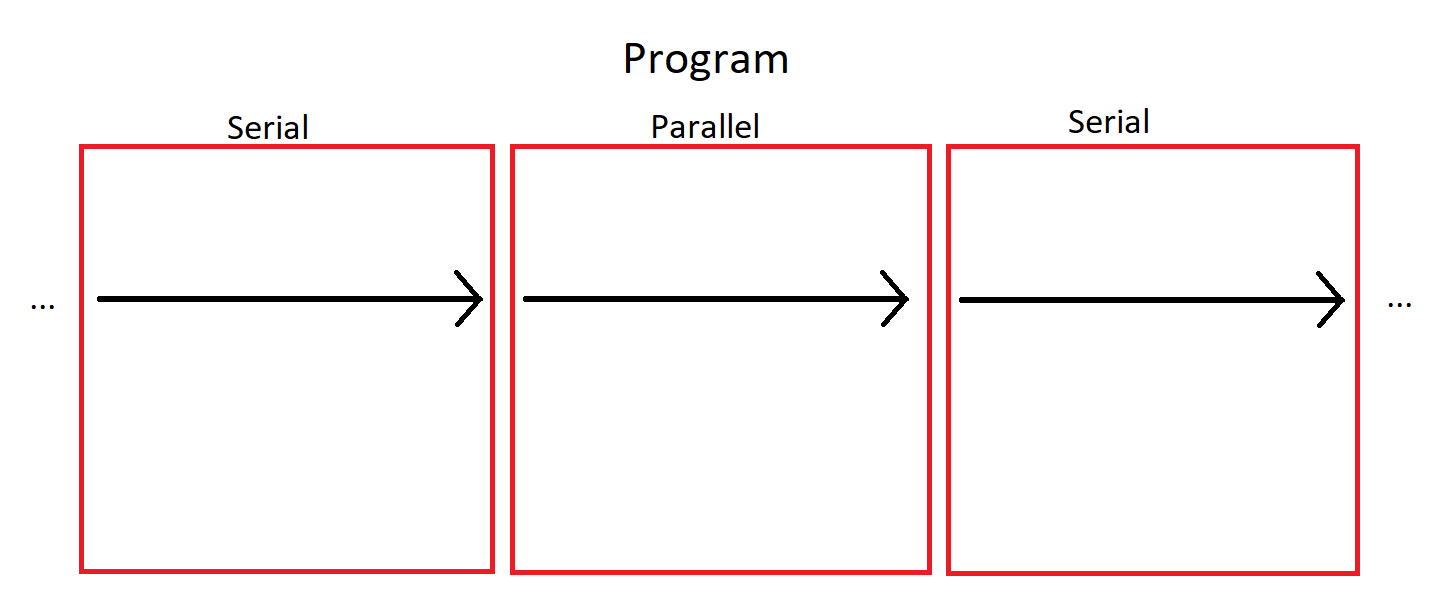
\includegraphics[width=\textwidth]{parallul.png}
	\caption{Programs have serial and parallel parts.}
	\end{figure}
\end{frame}
\begin{frame}{Parallel Computing}
Adding more resources at the wrong step will have no positive impact on overall performance. In fact it might cause problems.
	\begin{figure}
		\centering
		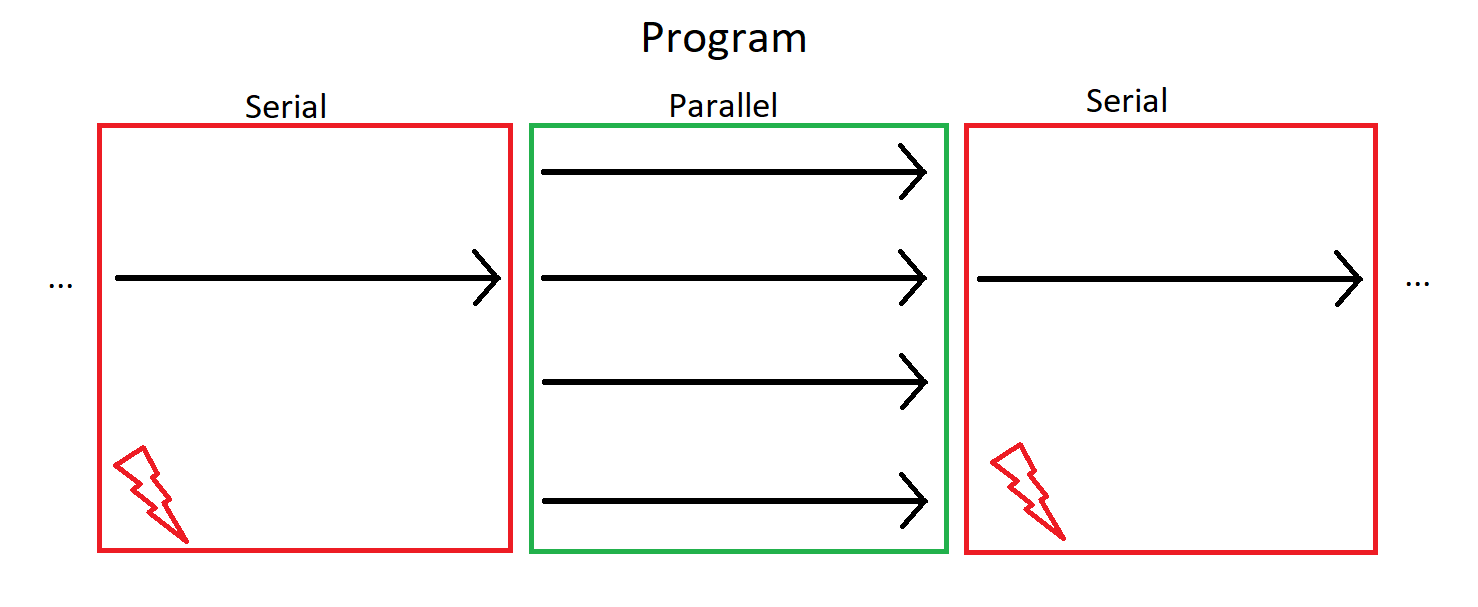
\includegraphics[width=\textwidth]{paraomegalul.png}
		\caption{Parallel parts benefit from more computing resources, serial parts don't.}
	\end{figure}
\end{frame}


\begin{frame}{Parallel Computing}
	There are multiple ways to parallelize your program:	
	\begin{enumerate}
		\item Vectorization
		\item \textbf{Multi-Processing}
		\item \textbf{Multi-Threading}
		\item Multi-Streaming with GPUs
	\end{enumerate}
	\begin{block}{Right tool for the job}
			Choosing the right parallelization for your program is important.  In these slides I will focus mainly on Multi-Processing and Multi-Threading.
	\end{block}

\end{frame}
\begin{frame}{Parallel Computing}
	\begin{block}{Split up your workload}
	Parallel Computing requires you to split up a \textbf{larger problem} into \textbf{smaller sub-problems}, which can be calculated independently.
	\end{block}

	
	\begin{block}{Vectors, Matrices, Tensors}
		Vectors, Matrices and Tensors operations can be parallelized very easily as each element can calculated independently from the others.
	\end{block}
	\begin{block}{Setup your data}
	Splitting up a large datasets into smaller independent datasets is key for parallel execution. Each dataset can be computed on different Nodes inside the cluster.
	\end{block}

\end{frame}

\begin{frame}{Parallel Computing}
Not every dataset can be split up in the same way. Each subset must be independently computable.
		\begin{figure}
		\centering
		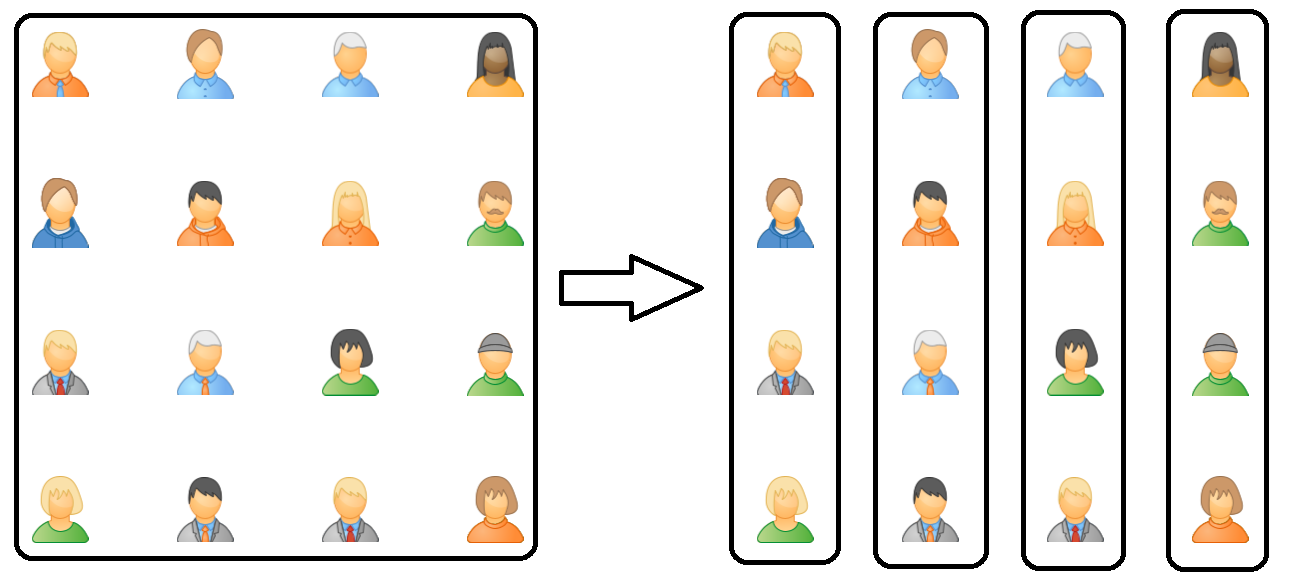
\includegraphics[width=\textwidth]{split_up.png}
		\caption{Splitting up a dataset of multiple subjects into smaller subsets.}
	\end{figure}
\end{frame}


\begin{frame}{Parallel Computing}
	\begin{itemize}
\item After splitting up your problem into smaller subsets, you can work on them in parallel
\item You can use multiple threads with a shared memory space to work with multiple cores on a single subset
\item You can use multiple processes with their own separate memory space to work with multiple cores on different subsets
	\end{itemize}


\end{frame}

\begin{frame}{Parallel Computing}
	Multi-Threading
	\begin{itemize}
		\item Memory is shared between multiple CPU-cores
		\item All CPU-cores work on the same variables
		\item Safety mechanisms for Race Conditions and Deadlocks can slow down computation
		\item Serial parts usually results in all but one CPU-cores are idling
	\end{itemize}
	Multi-Processing
	\begin{itemize}
		\item Multiple CPU-Cores work simultaneously in their own memory space
		\item Each CPU-Core has his own set of variables
		\item No slow down due to safety mechanisms or parallel parts
		\item No Perfomance gain for individual runtime
	\end{itemize}
	
	
\end{frame}

\begin{frame}{Parallel Computing}
	Using multiple threads can speed up the runtime of individual subsets. Multiple CPU-cores can work on the same data due to a shared memory space. During serial parts of your program, additional CPU-cores are idling.
	\begin{figure}
	\centering
	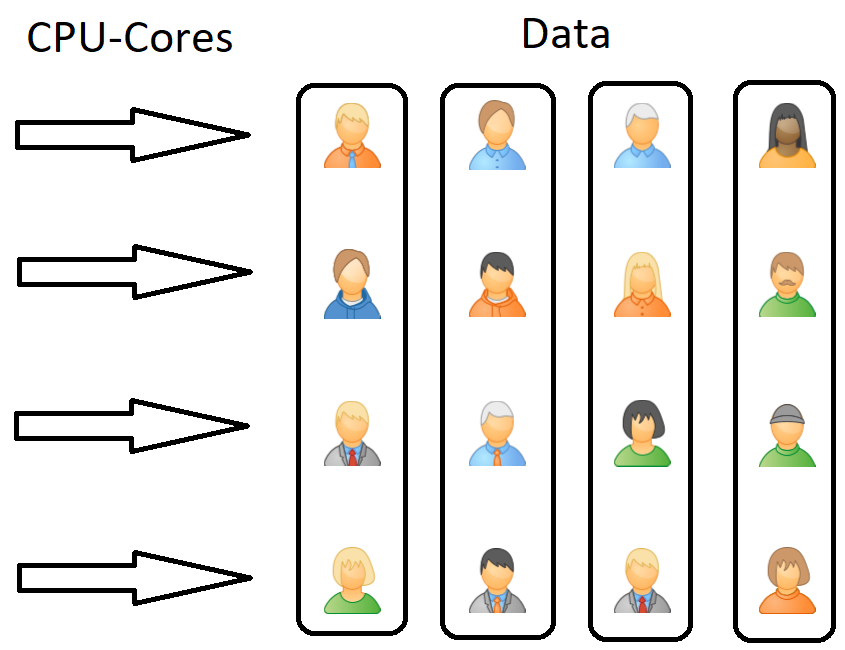
\includegraphics[width=0.5\textwidth]{thread.png}
	\caption{Multiple threads working together on the same subset.}
\end{figure}
\end{frame}

\begin{frame}{Parallel Computing}
		Using multiple processes doesn't speed up the runtime of individual subsets. However each process can run completely serially. No CPU-cores are idling during serial parts.
\begin{figure}
	\centering
	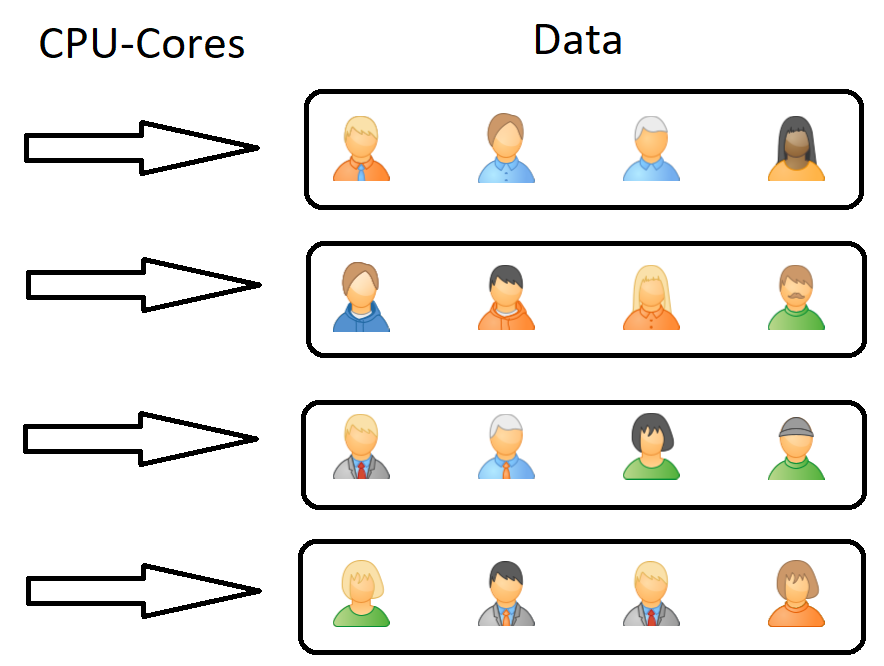
\includegraphics[width=0.5\textwidth]{process.png}
	\caption{Multiple processes work independently on different subsets.}
\end{figure}
\end{frame}

\begin{frame}{Parallel Computing}
	When to use multi-threading:
	\begin{itemize}
		\item Speeding up individual datasets, which can't be split up further/splitting up further is very hard.
		\item Individual runtime is very important.
		\item Your computation has very small serial parts/big parallel parts.
	\end{itemize}
	When to use multi-processing:
	\begin{itemize}
		\item Datasets can be split up into very small subsets
		\item Individual runtime is not important, overall runtime needs to be quick
		\item Your program doesn't benefit from a shared memory space
	\end{itemize}
	\begin{block}{Try out what works best}
		Parallel computing is very complex and requires a lot of testing. Try out different levels of parallezitaion and even combine both methods. Test your job-scripts on smaller subsets and look how they impact runtime.
	\end{block}
\end{frame}




% Main content frame
\section{Our HPC-Cluster}
\begin{frame}{Our HPC-Cluster}

	    \begin{itemize}
		\item 24 virtual nodes and many other hardware nodes (old hardware getting reused)
		\item Access via your RDS-Machines
		\item Local storage and Flstorage+Home shared
		\item Resources are CPU, RAM and GPU
	\end{itemize}
%    \begin{block}{Key Point 1}
%        Describe the first key point here.
%    \end{block}

%    \begin{block}{Key Point 2}
%        Describe the second key point here.
%    \end{block}
\end{frame}

% Conclusion frame
\section{Basic Tools}
\begin{frame}{Basic Tools}
    \begin{itemize}
        \item sinfo/squeue Status
        \item salloc/srun/sbatch Nutzung
        \item sacct Analyse
    \end{itemize}
\end{frame}

\section{Requesting Resources}
\begin{frame}{Requesting Resources}
	\begin{itemize}
		\item Default Values
		\item Absolute/relative
		\item CPU/RAM/GPU
	\end{itemize}
\end{frame}

\section{Using the cluster}
\begin{frame}{Interactive Mode}
	\begin{itemize}
		\item Interactive mode for testing
		\item srun to run commands on cluster
		\item salloc for longer session
	\end{itemize}
\end{frame}



\begin{frame}{Batch Processing}
	\begin{itemize}
		\item Kinit -> copy input -> process -> Kinit -> mv output
		\item Request ressources in script
		\item Mail
	\end{itemize}
\end{frame}

\section{Kerberos}
\begin{frame}{Kerberos}
	\begin{itemize}
		\item Kerberos on RDS (Login -> no manual kinit needed)
		\item Create Keytab
		\item Kinit in script
	\end{itemize}
\end{frame}

\section{Examples}
\begin{frame}{Examples}
	\begin{itemize}
		\item Normal
		\item Array
	\end{itemize}
\end{frame}
	% End of presentation
\begin{frame}
    \centering \Large
    Thank You!
\end{frame}
\end{document}
